\PassOptionsToClass{handout}{beamer}
\documentclass[biblatex]{cryptolecture}

\setbeamercovered{transparent}

\usepackage{amsmath,amsfonts,amssymb}
\usepackage{pgfplots}
\usepackage{mathtools}
\usepackage{bm}
\usepackage{xcolor,colortbl}
\usepackage{minted}
\usepackage{listings}
\usepackage{hyperref}
\usepackage{warp}

\usepackage{parskip}
\setlength{\parskip}{\medskipamount}

\tikzset{XOR/.style={draw,circle,scale=1,append after command={
        [shorten >=\pgflinewidth, shorten <=\pgflinewidth,]
        (\tikzlastnode.north) edge (\tikzlastnode.south)
        (\tikzlastnode.east) edge (\tikzlastnode.west)
        }
    }
}

% Names
% Algorithms (alphabetical)
\newcommand{\aes}{\cipher{AES}}
\newcommand{\aeslow}{\cipher{AES-128}}
\newcommand{\keccak}{\cipher{Keccak}}
\newcommand{\shathree}{\cipher{SHA-3}}

% Gates
\newcommand{\andg}{\texttt{AND}}
\newcommand{\org}{\texttt{OR}}
\newcommand{\nandg}{\texttt{NAND}}
\newcommand{\notg}{\texttt{NOT}}
\newcommand{\xorg}{\texttt{XOR}}
\newcommand{\copyg}{\texttt{COPY}}

% Customs (alphabetical)
\renewcommand{\cipher}[1]{\textsc{#1}}
\newcommand{\conc}{\mid \mid} % custom concat symbol
\newcommand{\emphteal}[1]{{\color{teal}#1}}
\newcommand{\emphred}[1]{{\color{red}#1}}
\newcommand{\ideal}{\text{Id}}
\newcommand{\midsized}{\;\middle|\;}

\newcommand{\z}{$\cdot$}
\newcommand{\es}{}
\renewcommand{\tabcolsep}{6pt}

\newcommand{\marknotcovered}{\begin{tikzpicture}[tugtheme]
  \draw (current page.east) node[rotate=90,gray!50,anchor=base,font=\bfseries\huge] {not covered 2024};
\end{tikzpicture}}

% Table coloring
\makeatletter
\def\rowcolor{\noalign{\ifnum0=`}\fi\bmr@rowcolor}
\newcommand<>{\bmr@rowcolor}{%
    \alt#1%
        {\global\let\CT@do@color\CT@@do@color\@ifnextchar[\CT@rowa\CT@rowb}% 
        {\ifnum0=`{\fi}\@gooble@rowcolor}% 
}

\newcommand{\@gooble@rowcolor}[2][]{\@gooble@rowcolor@}
\newcommand{\@gooble@rowcolor@}[1][]{\@gooble@rowcolor@@}
\newcommand{\@gooble@rowcolor@@}[1][]{\ignorespaces}
\makeatother

\begin{document}

\title{Algebraic Cryptanalysis}
\author{Hosein Hadipour\\[4pt]
% \tiny Partially based on slides by Maria Eichlseder
}

\date{Cryptanalysis -- ST 2024}
\web{www.iaik.tugraz.at/cryptanalysis}

%----------------------------------------------------------------------
\begin{frame}[plain,noframenumbering]
  \maketitle
\end{frame}
%----------------------------------------------------------------------
\section{Outside-in Approach in Algebraic Cryptanalysis}
\sectionheader[\huge\color{tug}$\int$]{Outside-in Approach in Algebraic Cryptanalysis}

\begin{frame}{Algebraic Cryptanalysis - Outside-in Approach}
\vspace{0.5cm}
\begin{figure}
\centering
\begin{tikzpicture}[node distance=2cm, auto]
  % Box styles
  \tikzstyle{box} = [rectangle, draw, fill=blue!20, text width=3cm, text centered, minimum height=2cm, rounded corners]
  % Arrow style
  \tikzstyle{arrow} = [thick,->,>=latex, rounded corners]
  
  % Nodes
  \node[box] (box1) {Cryptographic Primitive};
  \node[box, below=0.7cm of box1] (box2) {Constraint Programming};
  \node[box, right=2cm of $(box1.east)!0.5!(box2.east)$] (box3) {Investigate the Algebraic Structure};
  \node[box, right=2cm of box3] (box4) {Exploit The Weaknesses in Algebraic Structure};
  
  % Arrows
  \draw[arrow] (box1.east) -- ++(1cm,0) |- (box3.west);
  \draw[arrow] (box2.east) -- ++(1cm,0) |- (box3.west);
  \draw[arrow] (box3) -- (box4);
\end{tikzpicture}
\end{figure}
\begin{itemize}
  \item Integral attack
  \item Cube attack on stream ciphers and sponge functions
\end{itemize}
\end{frame}


\section{Symbolic Representation of Boolean Functions}
\sectionheader[\huge\color{tug}\faSuperscript]{Symbolic Representation of Boolean Functions}

\begin{frame}{Notations}
\begin{itemize}
	\item $\mathbb{F}_{2}$: Field with two elements
	\item $\mathbb{F}_{2}^{n}$: Vector space of dimension $n$ over $\mathbb{F}_{2}$
	\item $\bm{u} = (u_{0}, \cdots, u_{n - 1})$: Bit vectors in $\mathbb{F}_{2}^{2}$
	\item $\bm{e}_{i}$: $n$-bit unit vector with $1$ at position $i$ and $0$ elsewhere
	\item \textbf{A partial order over $\mathbb{F}_{2}^{n}$}: For any $\bm{u}, \bm{v} \in \mathbb{F}_{2}^{n}$: $\bm{u} \leq \bm{v}$ if $u_{i} \leq v_{i}$ for all $i$
	\item For all $\bm{x}, \bm{u}\in \mathbb{F}_{2}^{n}$: if $\bm{x} < \bm{u}$, then $\bm{x}^{\bm{u}} = 0$
	\item For all $\bm{x}, \bm{u}\in \mathbb{F}_{2}^{n}$: if $\bm{x} = \bm{u}$, then $\bm{x}^{\bm{u}} = 1$
	\item $\mathbb{F}_{2}[x_{0},\cdots, x_{n - 1}]$: Ring of polynomials with $n$ variables over $\mathbb{F}_{2}$
	\item Monomial: $\bm{x}^{\bm{u}} = \pi_{\bm{u}} (\bm{x}) = \prod_{i = 0}^{n - 1} x_{i}^{u_{i}}$, e.g., $(x_{2}, x_{1}, x_{0})^{(1, 0, 1)} = x_{2}x_{0}$
\end{itemize}
\end{frame}

\begin{frame}[fragile]
\frametitle{Different Representations of Boolean Functions}
\begin{columns}
\column{0.5\textwidth}
\begin{itemize}
  \item Truth Table (\texttt{TT})
  \vspace{0.2cm}
  \item Logical Expression
  \begin{itemize}
    \item\textcolor{tugred}{\texttt{CNF}}: $\begin{aligned}[t]
    &\left(x_2 \vee x_1 \vee \neg x_0\right) \wedge \left(x_2 \vee \neg x_1 \vee x_0\right) \wedge \\
    &\left(\neg x_2 \vee \neg x_1 \vee x_0\right) \wedge \left(\neg x_2 \vee \neg x_1 \vee \neg x_0\right)
    \end{aligned}$
    \vspace{0.15cm}
    \item\texttt{DNF}: $\begin{aligned}[t]
    &\left(\neg x_2 \wedge \neg x_1 \wedge \neg x_0\right) \vee \left(\neg x_2 \wedge x_1 \wedge x_0\right) \vee\\
    &\left(x_2 \wedge \neg x_1 \wedge \neg x_0\right) \vee \left(x_2 \wedge \neg x_1 \wedge x_0\right)
    \end{aligned}$
  \end{itemize}
  \vspace{0.2cm}
  \item Algebraic Normal Form (\textcolor{tugred}{\texttt{ANF}})
  \[f\left(x_2, x_1, x_0\right) = x_0 \cdot x_2 + x_0 + x_1 + 1\]
\end{itemize}
\column{0.5\textwidth}
\vspace{1cm}
\begin{table}
\centering
\begin{tabular}{|ccc|c|} 
\hline
\(x_2\) & \(x_1\) & \(x_0\)& \(f\) \\
\hline
\(0\) & \(0\) & \(0\) & \(1\) \\
\(0\) & \(0\) & \(1\) & \(0\) \\
\(0\) & \(1\) & \(0\) & \(0\) \\
\(0\) & \(1\) & \(1\) & \(1\) \\
\(1\) & \(0\) & \(0\) & \(1\) \\
\(1\) & \(0\) & \(1\) & \(1\) \\
\(1\) & \(1\) & \(0\) & \(0\) \\
\(1\) & \(1\) & \(1\) & \(0\) \\
\hline
\end{tabular}
\end{table}
\end{columns}
\end{frame}

\begin{frame}[fragile]
\frametitle{Algebraic Normal Form (ANF)}
\begin{block}{ANF}
A Boolean function $f:\mathbb{F}_{2}^{n}\rightarrow \mathbb{F}_{2}$ 
can be uniquely represented by a polynomial in 
$\frac{\mathbb{F}_{2}[x_{0}, \ldots, x_{n - 1}]}{\langle x_{0}^{2} + x_{0}, \ldots, x_{n - 1}^{2} + x_{n - 1}\rangle}$:
\[
	f(\bm{x}) = \sum_{\bm{u}\in \mathbb{F}_{2}^{n}} a_{\bm{u}} \cdot \bm{x}^{\bm{u}}, \quad \text{where} \quad a_{\bm{u}}\in \mathbb{F}_{2},\, \text{and}\;\bm{x}^{\bm{u}} = x_{0}^{u_{0}}\cdots x_{n - 1}^{u_{n - 1}}.
\]
\end{block}
\begin{itemize}
\item[\faCheckCircle] If $f(\bm{x}) = \sum_{\bm{u}\in \mathbb{F}_{2}^{n}} a_{\bm{u}}\cdot \bm{x}^{\bm{u}}$, and $\bm{x} \leq \bm{u}$ iff $x_{i} \leq u_{i}$ for all $i$, then for all $\bm{u} \in \mathbb{F}_{2}^{n}$:
\begin{itemize}
	\item[\faCheckCircle] \colorbox{tug!30}{$a_{\bm{u}} = \sum_{\bm{x} \leq \bm{u}} f(\bm{x})$}
	\item[\faCheckCircle] $f(\bm{u}) = \sum_{\bm{x} \leq \bm{u}} a_{\bm{x}}$
\end{itemize}
\end{itemize}
\end{frame}

\begin{frame}[fragile]{Relations Between Coefficients and (Sum of the) Outputs}
\vspace{-0.4cm}
\begin{itemize}
\item If $f(\bm{x}) = \sum_{\bm{u}\in \mathbb{F}_{2}^{n}} a_{\bm{u}}\cdot \bm{x}^{\bm{u}}$, then for all $\bm{u} \in \mathbb{F}_{2}^{n}$:\\
\begin{itemize}
	\item \colorbox{tug!30}{$a_{\bm{u}} = \sum_{\bm{x} \leq \bm{u}} f(\bm{x})$} \hspace*{2cm}
	\item $f(\bm{u}) = \sum_{\bm{x} \leq \bm{u}} a_{\bm{x}}$
\end{itemize}
\end{itemize}
\pause
\vspace{0.7cm}
\begin{columns}
\column[c]{0.4\textwidth}
\centering
\begin{tabular}{cc|c}
$x_{1}$ & $x_{0}$ & $f(x_{1}, x_{0})$\\
\toprule
\rowcolor<3-6|handout:3-6>{colB!50} 0 & 0 & 1\\
\rowcolor<4,6|handout:4,6>{colB!50} 0 & 1 & 0\\
\rowcolor<5,6|handout:5,6>{colB!50} 1 & 0 & 1\\
\rowcolor<6,6|handout:6,6>{colB!50} 1 & 1 & 1
\end{tabular}
\column[c]{0.6\textwidth}
\centering
\begin{itemize}
\item<3-|handout:3-> $a_{(0, 0)} = \sum_{u \leq (0, 0)} f(x) = 1 \;\textcolor{tugred}{\Rightarrow 1 \rightarrow f}$
\item<4-|handout:4-> $a_{(0, 1)} = \sum_{u \leq (0, 1)} f(x) = 1 \;\textcolor{tugred}{\Rightarrow x_0 \rightarrow f}$
\item<5-|handout:5-> $a_{(1, 0)} = \sum_{u \leq (1, 0)} f(x) = 0 \;\textcolor{tugred}{\Rightarrow x_1 \not\rightarrow f}$
\item<6-|handout:6-> $a_{(1, 1)} = \sum_{u \leq (1, 1)} f(x) = 1 \;\textcolor{tugred}{\Rightarrow x_1 x_0 \rightarrow f}$
\end{itemize}
\end{columns}
\vspace{0.3cm}
{\large
\[f(x_{1}, x_{0}) = \visible<3-|handout:3->{1 + }
                    \visible<4-|handout:4->{x_{0} + }
                    \visible<5-|handout:5->{\textcolor{gray}{x_{1}} + }
                    \visible<6-|handout:6->{ x_{1} x_{0}}\]
}
\end{frame}

\begin{frame}[fragile]
\frametitle{Deriving \texttt{ANF} in SageMath}
\begin{overprint}
\small
% \onslide<2>
% \begin{minted}[linenos,highlightlines={4}]{python}
% from sage.crypto.boolean_function import BooleanFunction as BF            
% f = BF([0, 0, 0, 1])
% g = f.algebraic_normal_form(); g #x0: LSB                                  
% x0*x1 
% \end{minted}
% \onslide<3>
\begin{minted}[linenos,highlightlines={4, 6, 8, 10}]{python}
sage: from sage.crypto.boolean_function import BooleanFunction as BF            
sage: f = BF([0, 0, 1, 1, 0, 1, 0, 1, 0, 1, 0, 1, 0, 1, 0, 1])
sage: g = f.algebraic_normal_form(); g
x0*x2*x3 + x0*x2 + x0*x3 + x1*x2*x3 + x1*x2 + x1*x3 + x1
sage: g.variables()
(x0, x1, x2, x3)
sage: g.monomials()
[x0*x2*x3, x0*x2, x0*x3, x1*x2*x3, x1*x2, x1*x3, x1]
sage: g.degree()
3
\end{minted}
\end{overprint}
\end{frame}

\section{Integral Distinguishers From the Algebraic Perspective}
\sectionheader[\huge\color{tug}\faEye\,$\sum$]{Integral Distinguishers From the\\ Algebraic Perspective}

\begin{frame}[fragile]{Integral Distinguisher and The Coefficients of ANF}
\begin{columns}
\column[c]{0.7\textwidth}
\begin{itemize}
\small
\item<1->[\faConnectdevelop] $y=f(\bm{k}, \bm{x}) \only<1>{= \sum_{\bm{u}\in \mathbb{F}_{2}^{n}} \sum_{\bm{v}\in \mathbb{F}_{2}^{k}} a_{\bm{u},\bm{v}}\bm{k}^{\bm{v}} \bm{x}^{\bm{u}}} \only<2->{= \sum_{\bm{u}\in \mathbb{F}_{2}^{n}} \textcolor{tugred}{a_{\bm{u}}(\bm{k})}\cdot \bm{x}^{\bm{u}}}$
\vspace{0.5cm}
\item<3->[\faCube] $\mathbb{C}_{\bm{u}} = \{x \in \mathbb{F}_{2}^{n}\,|\, \bm{x} \leq \bm{u}\}$
\vspace{0.5cm}
\item<4->[\faCheckCircle] $\textcolor{tugred}{a_{\bm{u}}(\bm{k}) = \sum_{\bm{x} \leq \bm{u}} f(\bm{k},\bm{x})}$
\vspace{0.5cm}
\item<5->[\faBell]
Which monomial is key-independent in the ANF?
\begin{itemize}
\vspace{0.3cm}
\item[\faGem] zero-sum: $\exists\, u,\, s.t.\, \forall \bm{k}:\, a_{\bm{u}}(\bm{k}) = 0$
\hspace*{2cm}
\vspace{0.5cm}
\item[\faGem] one-sum: $\ \exists\, u,\, s.t. \, \forall \bm{k}:\,a_{\bm{u}}(\bm{k}) = 1$
\end{itemize}
\end{itemize}
\column[c]{0.3\textwidth}
\begin{overprint}
\begin{tikzpicture}[yscale=1.3, xscale=1.3, thick,
every node/.style={inner sep=5pt},
next/.append style={rounded corners=3pt},
primi/.append style={fill=tugred!50, draw=black, rounded corners=2pt, minimum size=30pt},
caption/.style={gray, below=1.75cm, align=center}]
\pgfmathsetmacro{\cubex}{1.5}
\pgfmathsetmacro{\cubey}{1.5}
\pgfmathsetmacro{\cubez}{1.5}
\visible<3->{
\draw[tuggray,fill=tugblue!50,opacity=0.5] (0.5,+2.5,0) -- ++(-\cubex,0,0) -- ++(0,-\cubey,0) -- ++(\cubex,0,0) -- cycle;
\draw[tuggray,fill=tugblue!50,opacity=0.5] (0.5,+2.5,0) -- ++(0,0,-\cubez) -- ++(0,-\cubey,0) -- ++(0,0,\cubez) -- cycle;
\draw[tuggray,fill=tugblue!50] (0.5,+2.5,0) -- ++(-\cubex,0,0) -- ++(0,0,-\cubez) -- ++(\cubex,0,0) -- cycle;}
\node[primi, key west] (E) {$E$};
\draw[next]  (E) ++(0,1.5) node[above] {$\bm{x}$\,\faFile*} -- (E);
\draw[next]  (E) ++(-1,0) node[above] {$\bm{k}$\,\faKey} -- (E);
\draw[prev]  (E) ++(0,-1.5) node[below] {
  \only<1-3>{
  $y$\,\faEnvelope}
    \only<4->{
    \textcolor{tugred}{$\textcolor{tugred}{\sum_{\bm{x} \leq \bm{u}} f(\bm{k},\bm{x})}$}}
} -- (E);
%\pause
\end{tikzpicture}
\end{overprint}
\end{columns}
\end{frame}

\section{Monomial Prediction and Our SAT Model}
\sectionheader[\huge\color{tug}\faCogs]{Monomial Prediction and Our SAT Model}

\begin{frame}{Core Idea of Monomial Prediction \cite{monomial_prediction_asiacrypt_HuSW020}}
\begin{figure}
\resizebox{0.8\textwidth}{!}{%
\begin{tikzpicture}[xscale=1,yscale=1,very thin,>=latex]
	\coordinate (here) at (0, 0);
	\node[box, right=1cm of here] (R) {$\bm{f}_{1}$};
	\node[xor, right=0.5cm of R] (AK) {};
	\coordinate[above=1.5cm of AK] (RKSource);
	\node[right=1cm of AK] (DOTS){$\cdots$};
	\draw[next] (here) -- (R);
	\node[] at ($(here) + (0.25, -0.31)$) {$\bm{x}$};
	\draw[next] (R) -- (AK);
	\draw[next] (AK) -- (DOTS);
	\node[] at ($(AK) + (0.7, -0.31)$) {};
	\draw[next] (RKSource) -- node[anchor=east] {} (AK);
	\draw[fill opacity = 1, rounded corners=1mm, dashed] ($(here) + (0.78, -0.5)$) rectangle ($(here) + (2.65, 0.55)$);
	\coordinate[right=1pt of DOTS] (here);
	\coordinate (T1) at ($(AK.north) + (-0.5, 1.5)$) {};
	\coordinate (T4) at ($(AK.north) + (0.5, 2.5)$) {};
	\coordinate (K0_1) at ($(AK.north) + (-2.4, 2)$);
	\coordinate (K0_2) at ($(AK.north) + (0, 2)$);
	\draw[next, rounded corners=1mm] (K0_1) -- node[anchor=north] {$\bm{k}$} (K0_2);

	\node[box, right=1cm of here] (R) {$\bm{f}_{i}$};
	\node[xor, right=0.5cm of R] (AK) {};
	\coordinate[above=1.5cm of AK] (RKSource);
	\node[right=1cm of AK] (DOTS){$\cdots$};
	\draw[next] (here) -- (R);
	\node[] at ($(here) + (0.25, -0.31)$) {};
	\draw[next] (R) -- (AK);
	\draw[next] (AK) -- (DOTS);
	\node[] at ($(AK) + (0.7, -0.31)$) {};
	\draw[next] (RKSource) -- node[anchor=east] {} (AK);
	\draw[fill opacity = 1, rounded corners=1mm, dashed] ($(here) + (0.78, -0.5)$) rectangle ($(here) + (2.65, 0.55)$);
	\coordinate[right=1pt of DOTS] (here);
	\node[above=1.7cm of AK] {Key Schedule};

	\node[box, right=1cm of here] (R) {$\bm{f}_{r}$};
	\node[xor, right=0.5cm of R] (AK) {};
	\coordinate[above=1.5cm of AK] (RKSource);
	\node[right=1cm of AK] (DOTS){};
	\draw[next] (here) -- (R);
	\node[next] at ($(here) + (0.25, -0.31)$) {};
	\draw[next] (R) -- (AK);
	\draw[next] (AK) -- (DOTS);
	\node[] at ($(AK) + (0.7, -0.31)$) {$\bm{y}$};
	\draw[next] (RKSource) -- node[anchor=east] {} (AK);
	\draw[fill opacity = 1, rounded corners=1mm, dashed] ($(here) + (0.78, -0.5)$) rectangle ($(here) + (2.65, 0.55)$);
	\coordinate[right=1pt of DOTS] (here);

	\coordinate (T2) at ($(AK.north) + (+0.5, 1.5)$) {};
	\coordinate (T3) at ($(AK.north) + (-0.5, 2.5)$) {};

	\draw[rounded corners=1mm] (T1) -- (T2) -- (T3) -- (T4) -- cycle;
\end{tikzpicture}
}
\end{figure}
\vspace{0.5cm}
\begin{block}{Core Idea}
The absence (or presence) of a monomial in the ANF of a composite function can be checked by 
tracking the propagation of the given monomial through the building blocks of composite functions.
\end{block}
\end{frame}

\begin{frame}{Monomial Trail and Integral Distinguisher}
\footnotesize
\begin{overprint}
\onslide<1-|handout:1->{%
\begin{figure}
\resizebox{0.8\textwidth}{!}{%
\begin{tikzpicture}[xscale=1,yscale=1,very thin,>=latex]
  \coordinate (here) at (0, 0);
  \node[box, right=1cm of here] (R) {$\bm{f}_{1}$};
  \node[xor, right=0.5cm of R] (AK) {};
  \coordinate[above=1.5cm of AK] (RKSource);
  \node[right=1cm of AK] (DOTS){$\cdots$};
  \draw[next] (here) -- (R);
  \node[] at ($(here) + (0.25, -0.31)$) {$\bm{x}^{\bm{u}}$};
  \draw[next] (R) -- (AK);
  \draw[next] (AK) -- (DOTS);
  \node[] at ($(AK) + (0.7, -0.31)$) {$\bm{s}^{\bm{\alpha}}$};
  \draw[next] (RKSource) -- node[anchor=east] {} (AK);
  \draw[fill opacity = 1, rounded corners=1mm, dashed] ($(here) + (0.78, -0.5)$) rectangle ($(here) + (2.65, 0.55)$);
  \coordinate[right=1pt of DOTS] (here);
  \coordinate (T1) at ($(AK.north) + (-0.5, 1.5)$) {};
  \coordinate (T4) at ($(AK.north) + (0.5, 2.5)$) {};
  \coordinate (K0_1) at ($(AK.north) + (-2.4, 2)$);
  \coordinate (K0_2) at ($(AK.north) + (0, 2)$);
  \draw[next, rounded corners=1mm] (K0_1) -- node[anchor=north] {$\bm{k}^{\bm{w}}$} (K0_2);

  \node[box, right=1cm of here] (R) {$\bm{f}_{i}$};
  \node[xor, right=0.5cm of R] (AK) {};
  \coordinate[above=1.5cm of AK] (RKSource);
  \node[right=1cm of AK] (DOTS){$\cdots$};
  \draw[next] (here) -- (R);
  \node[] at ($(here) + (0.25, -0.31)$) {};
  \draw[next] (R) -- (AK);
  \draw[next] (AK) -- (DOTS);
  \node[] at ($(AK) + (0.7, -0.31)$) {};
  \draw[next] (RKSource) -- node[anchor=east] {} (AK);
  \draw[fill opacity = 1, rounded corners=1mm, dashed] ($(here) + (0.78, -0.5)$) rectangle ($(here) + (2.65, 0.55)$);
  \coordinate[right=1pt of DOTS] (here);
  \node[above=1.7cm of AK] {Key Schedule};

  \node[box, right=1cm of here] (R) {$\bm{f}_{r}$};
  \node[xor, right=0.5cm of R] (AK) {};
  \coordinate[above=1.5cm of AK] (RKSource);
  \node[right=1cm of AK] (DOTS){};
  \draw[next] (here) -- (R);
  \node[next] at ($(here) + (0.25, -0.31)$) {$\bm{t}^{\bm{\beta}}$};
  \draw[next] (R) -- (AK);
  \draw[next] (AK) -- (DOTS);
  \node[] at ($(AK) + (1, -0.31)$) {$\bm{y}^{\bm{v}}$};
  \draw[next] (RKSource) -- node[anchor=east] {} (AK);
  \draw[fill opacity = 1, rounded corners=1mm, dashed] ($(here) + (0.78, -0.5)$) rectangle ($(here) + (2.65, 0.55)$);
  \coordinate[right=1pt of DOTS] (here);

  \coordinate (T2) at ($(AK.north) + (+0.5, 1.5)$) {};
  \coordinate (T3) at ($(AK.north) + (-0.5, 2.5)$) {};

  \draw[rounded corners=1mm] (T1) -- (T2) -- (T3) -- (T4) -- cycle;
\end{tikzpicture}
}
\end{figure}
}
\only<2-3|handout:1>{
{\large\[\bm{k}^{\bm{w}} \bm{x}^{\bm{u}} \xrightarrow{f_{1}} \bm{s}^{\bm{\alpha}} \xrightarrow{f_{2}} \cdots \xrightarrow{f_{i}} \cdots \xrightarrow{f_{r - 1}} \bm{t}^{\bm{\beta}} \xrightarrow{f_{r}} \bm{y}^{\bm{v}}\]}
\only<3|handout:1>{
{\large\[\bm{k}^{\bm{w}} \bm{x}^{\bm{u}} \rightsquigarrow \bm{y}^{\bm{v}}\]}
}
}
\only<4|handout:2>{
{\large\[\bm{k}^{\bm{w}} \bm{x}^{\bm{u}} \rightarrow \bm{y}^{\bm{v}} \Rightarrow \textcolor{tugred}{\bm{k}^{\bm{w}} \bm{x}^{\bm{u}} \rightsquigarrow \bm{y}^{\bm{v}}}\]}
}
\only<5|handout:2>{
  {\large\[\textcolor{tugred}{\bm{k}^{\bm{w}} \bm{x}^{\bm{u}} \not\rightsquigarrow \bm{y}^{\bm{v}}} \Rightarrow \bm{k}^{\bm{w}} \bm{x}^{\bm{u}} \not\rightarrow \bm{y}^{\bm{v}}\]}
}
\visible<6-|handout:3->{
\[\bm{y}^{\bm{v}} = \sum_{\bm{u}\in \mathbb{F}_{2}^{n}} \sum_{\bm{v}\in \mathbb{F}_{2}^{k}} a_{\bm{u},\bm{v}}\bm{k}^{\bm{v}} \bm{x}^{\bm{u}} = \sum_{\bm{u}\in \mathbb{F}_{2}^{n}} \textcolor{tugred}{a_{\bm{u}}(\bm{k})} \cdot \bm{x}^{\bm{u}}\]
\vspace{-0.3cm}
\begin{block}{From Monomial Trails to Integral Distinguisher}
\begin{itemize}
  \item<7-|handout:3>[\faBomb] If $\exists \bm{u}$ s.t. $\bm{k}^{\bm{w}} \bm{x}^{\bm{u}}\not\rightsquigarrow \bm{y}^{\bm{v}}$ for all $\bm{w} \in \mathbb{F}_{2}^{k}$ then \textcolor{tugred}{$a_{\bm{u}}(\bm{k}) = 0$}
  \item<8-|handout:3>[\faBomb] If $\exists \bm{u}$ s.t. $\bm{k}^{\bm{w}} \bm{x}^{\bm{u}}\not\rightsquigarrow \bm{y}^{\bm{v}}$ for all $\bm{w} \in \mathbb{F}_{2}^{k}\setminus \{\bm{0}\}$ then \textcolor{tugred}{$a_{\bm{u}}(\bm{k}) = \texttt{constant}$}
\end{itemize}
\end{block}
}
\end{overprint}
\end{frame}

\begin{frame}{From Monomial Prediction to SAT Problem}
\begin{columns}[T]
\column{0.5\textwidth}
\centering
\begin{tikzpicture}
\pgfmathsetmacro{\basicstep}{2}
\node[box, key north, minimum size=30pt, fill=tugred!50] (E) {$E$};
\draw[next] (E) ++(-\basicstep, 0) node[left] {$\bm{x}^{\bm{u}}$} -- (E) node[midway, above]{$n$} node[pos=0.55]{$\slash$};
\draw[prev] (E) ++(\basicstep, 0) node[right] {$\bm{y}^{\bm{v}}$} -- (E) node [midway, above]{$n$} node[pos=0.46]{$\slash$};
\draw[next, rounded corners=2pt] (E) ++(-\basicstep, \basicstep/2) node[left] {$\bm{k}^{\bm{w}}$} -| (E) node[pos=0.2, above]{$k$} node[pos=0.22]{$\slash$};
\end{tikzpicture}
\column{0.5\textwidth}
\centering
\null
\[\bm{y}^{\bm{v}} = \sum_{\bm{u}\in \mathbb{F}_{2}^{n}} \sum_{\bm{v}\in \mathbb{F}_{2}^{k}} a_{\bm{u},\bm{v}}\bm{k}^{\bm{v}} \bm{x}^{\bm{u}} = \sum_{\bm{u}\in \mathbb{F}_{2}^{n}} \textcolor{tugred}{a_{\bm{u}}(\bm{k})} \cdot \bm{x}^{\bm{u}}\]
\end{columns}
\vspace{0.5cm}
\begin{itemize}
\footnotesize
\item<1->[\faCodeBranch] \only<6>{\textcolor{tugblue}}{Model the propagation of monomial trails through the building blocks by a \texttt{CNF} clause}
\vspace{0.2cm}
\item<2->[\faBullhorn] Main variables are the monomial exponents, i.e., $\bm{u}, \bm{w}, \bm{v}, \ldots$ not $\bm{x}, \bm{k}, \bm{y}, \ldots$
\vspace{0.2cm}
\item<3->[\faAnchor] Fix $\bm{u}$ to a certain vector and set $\bm{v}$ to $\bm{e}_{i}$ ($\bm{w}$ should be a free variable but non-zero)
\vspace{0.2cm}
\item<4->[\faRoad] Any possible solution of the model is a monomial trail from $\bm{k}^{\bm{w}}\bm{x}^{\bm{u}}$ to  $\bm{y}^{\bm{v}}$
\vspace{0.2cm}
\item<5->[\faFlag] If the model is impossible, then $\bm{k}^{\bm{w}} \bm{x}^{\bm{u}}\not\rightsquigarrow \bm{y}^{\bm{v}}$ for all $\bm{w} \in \mathbb{F}_{2}^{k}$, and \textcolor{tug}{$a_{\bm{u}}(\bm{k}) = \texttt{constant}$}
\end{itemize}
\end{frame}

\begin{frame}{Monomial Prediction Table (\texttt{MPT})}
\begin{itemize}
\item[\faChevronCircleRight]
Let $\bm{y} = \bm{f}(\bm{x})$ be an $m$-bit to $n$-bit vectorial Boolean function. Then $\texttt{MPT}(\bm{u}, \bm{v}) = 1$ if $\bm{x}^{\bm{u}} \xrightarrow{f} \bm{y}^{\bm{v}}$, and $\texttt{MPT}(\bm{u}, \bm{v}) = 0$ otherwise.
\end{itemize}
\vspace{0.25cm}
\begin{columns}
\scriptsize
\column[c]{0.2\textwidth}
\centering
\only<2-|handout:1->{
\resizebox{0.5\textwidth}{!}{
\begin{tabular}{c|l}
$x$ &\!$S(x)$\\
\toprule
\texttt{0} & \texttt{c}\\
\texttt{1} & \texttt{a}\\
\texttt{2} & \texttt{d}\\
\texttt{3} & \texttt{3}\\
\texttt{4} & \texttt{e}\\
\texttt{5} & \texttt{b}\\
\texttt{6} & \texttt{f}\\
\texttt{7} & \texttt{7}\\
\texttt{8} & \texttt{8}\\
\texttt{9} & \texttt{9}\\
\texttt{a} & \texttt{1}\\
\texttt{b} & \texttt{5}\\
\texttt{c} & \texttt{0}\\
\texttt{d} & \texttt{2}\\
\texttt{e} & \texttt{4}\\
\texttt{f} & \texttt{6}\\
\end{tabular}}
}
\column[c]{0.8\textwidth}
\centering
\only<3|handout:1>{
\resizebox{0.75\textwidth}{!}{
\begin{tabular}{r|*{16}{r}}
  \toprule
  $\bm{u}$\,\textbackslash\,$\bm{v}$ & \es\texttt{0}\es & \es\texttt{1}\es & \es\texttt{2}\es & \es\texttt{3}\es & \es\texttt{4}\es & \es\texttt{5}\es & \es\texttt{6}\es & \es\texttt{7}\es & \es\texttt{8}\es & \es\texttt{9}\es & \es\texttt{a}\es & \es\texttt{b}\es & \es\texttt{c}\es & \es\texttt{d}\es & \es\texttt{e}\es & \es\texttt{f}\es \\
  \midrule
  \texttt{0\,} &  1 & \z & \z & \z &  1 & \z & \z & \z &  1 & \z & \z & \z &  1 & \z & \z & \z\\
  \texttt{1\,} & \z & \z &  1 & \z &  1 & \z & \z & \z & \z & \z &  1 & \z &  1 & \z & \z & \z\\
  \texttt{2\,} & \z &  1 & \z & \z & \z &  1 & \z & \z & \z &  1 & \z & \z & \z &  1 & \z & \z\\
  \texttt{3\,} & \z & \z & \z &  1 & \z &  1 & \z & \z &  1 &  1 &  1 & \z & \z &  1 & \z & \z\\
  \texttt{4\,} & \z & \z &  1 & \z & \z & \z &  1 & \z & \z & \z &  1 & \z & \z & \z &  1 & \z\\
  \texttt{5\,} & \z &  1 &  1 &  1 & \z & \z &  1 & \z & \z &  1 &  1 &  1 & \z & \z &  1 & \z\\
  \texttt{6\,} & \z & \z & \z &  1 & \z & \z & \z &  1 & \z & \z & \z &  1 & \z & \z & \z &  1\\
  \texttt{7\,} & \z &  1 & \z & \z &  1 &  1 &  1 & \z & \z &  1 & \z & \z & \z & \z & \z &  1\\
  \texttt{8\,} & \z & \z & \z & \z &  1 & \z & \z & \z & \z & \z & \z & \z &  1 & \z & \z & \z\\
  \texttt{9\,} & \z &  1 &  1 & \z &  1 & \z & \z & \z & \z &  1 &  1 & \z &  1 & \z & \z & \z\\
  \texttt{a\,} & \z & \z & \z & \z & \z &  1 & \z & \z &  1 &  1 & \z & \z & \z &  1 & \z & \z\\
  \texttt{b\,} & \z &  1 & \z &  1 &  1 & \z & \z & \z &  1 & \z &  1 & \z & \z &  1 & \z & \z\\
  \texttt{c\,} & \z & \z &  1 & \z & \z & \z &  1 & \z &  1 & \z &  1 & \z & \z & \z &  1 & \z\\
  \texttt{d\,} & \z & \z & \z &  1 & \z & \z &  1 & \z & \z & \z &  1 &  1 & \z & \z &  1 & \z\\
  \texttt{e\,} & \z &  1 & \z &  1 &  1 & \z & \z &  1 &  1 & \z & \z &  1 & \z & \z & \z &  1\\
  \texttt{f\,} & \z & \z & \z & \z & \z & \z & \z & \z & \z & \z & \z & \z & \z & \z & \z &  1\\
  \bottomrule
\end{tabular}}
}
\only<4-|handout:2>
{
{\tiny
\begin{align*}
& \quad  (u_2 \vee \neg v_1 \vee \neg v_3) &                    & \wedge (\neg u_1 \vee \neg v_0 \vee \neg v_1 \vee v_2) &              & \wedge (\neg u_0 \vee \neg u_1 \vee \neg u_2 \vee \neg v_2 \vee v_3) \\
& \wedge (u_2 \vee u_3 \vee \neg v_3) &                         & \wedge (\neg u_0 \vee \neg u_1 \vee \neg u_3 \vee v_2) &              & \wedge (\neg u_0 \vee \neg u_3 \vee v_0 \vee \neg v_1 \vee \neg v_3) \\
& \wedge (u_1 \vee \neg v_1 \vee \neg v_2) &                    & \wedge (\neg u_1 \vee u_2 \vee v_0 \vee v_2 \vee v_3) &               & \wedge (\neg u_0 \vee \neg u_1 \vee \neg u_3 \vee v_0 \vee v_1 \vee v_3) \\
& \wedge (u_1 \vee u_3 \vee \neg v_2) &                         & \wedge (u_2 \vee \neg u_3 \vee v_1 \vee v_2 \vee v_3) &               & \wedge (\neg u_0 \vee \neg u_2 \vee \neg u_3 \vee \neg v_0 \vee v_1 \vee \neg v_3) \\
& \wedge (u_0 \vee \neg u_2 \vee u_3 \vee v_3) &                & \wedge (u_1 \vee \neg v_0 \vee \neg v_2 \vee \neg v_3) &              & \wedge (\neg u_1 \vee \neg u_2 \vee \neg u_3 \vee v_1 \vee \neg v_2) \\
& \wedge (u_0 \vee \neg u_1 \vee u_3 \vee v_2) &                & \wedge (\neg u_0 \vee u_1 \vee u_3 \vee v_0 \vee v_1) &               & \wedge (\neg u_1 \vee \neg u_2 \vee \neg u_3 \vee v_1 \vee v_3) \\
& \wedge (\neg u_2 \vee v_0 \vee v_1 \vee v_3) &                & \wedge (\neg u_1 \vee u_3 \vee \neg v_0 \vee v_2 \vee \neg v_3)\!\!\!&& \wedge (u_0 \vee u_1 \vee \neg u_3 \vee v_0 \vee v_1 \vee v_2) \\
& \wedge (u_0 \vee u_1 \vee u_2 \vee \neg v_3) &                & \wedge (u_0 \vee u_1 \vee \neg u_2 \vee \neg v_1 \vee v_3) &          & \wedge (\neg u_3 \vee v_0 \vee \neg v_1 \vee \neg v_2 \vee \neg v_3) \\
& \wedge (u_1 \vee u_2 \vee \neg v_2 \vee \neg v_3) &           & \wedge (u_1 \vee \neg u_2 \vee u_3 \vee \neg v_1 \vee v_3) &          & \wedge (\neg u_0 \vee u_1 \vee u_2 \vee v_1 \vee v_2 \vee v_3) \\
& \wedge (\neg u_2 \vee \neg v_0 \vee \neg v_1 \vee v_3)\!\!\!& & \wedge (\neg u_1 \vee u_3 \vee \neg v_1 \vee v_2 \vee \neg v_3).\!\!\!
\end{align*}
}
\begin{itemize}
\item[\faGithub] {\footnotesize Sbox Analyzer: \url{https://github.com/hadipourh/sboxanalyzer}}
\end{itemize}
}
\end{columns}
\end{frame}

\section{Application to Integral Analysis of WARP}
\sectionheader[\huge\color{tug}\faTh]{Application to Integral Analysis\\ of WARP}

\begin{frame}{WARP\cite{sacrypt_BanikBIKLMSSS20}}
\begin{itemize}
	\footnotesize
	\item[\faArrowCircleRight] Proposed in SAC 2020 \cite{sacrypt_BanikBIKLMSSS20} as the lightweight alternative of \cipher{AES-128}
	\item[\faArrowCircleRight] 128-bit block/key size, and 41 rounds (40.5 rounds)
	\item[\faArrowCircleRight] Splits 128-bit $K$ into two halves $K^{(0)}||K^{(1)}$ and uses $K^{(r-1 \mod 2)}$ in the $r$th round
\end{itemize}
\begin{figure} % WARP round function %{{{
%\null\hskip-4pt%
\centering		
\begin{tikzpicture}[xscale=.45,yscale=.48,thin,>=latex,every node/.style={font=\tiny,inner sep=1pt}]
\coordinate (ptop) at (0,-3);
\coordinate (pbot) at (0,-5.5);
\foreach \z [evaluate=\z as \zz using int(2*\z), evaluate=\z as \zzz using int(2*\z+1)] in {0,...,15} {
  \draw (\zz,0)   node[above] {$X_{\zz}$}   ++(-.25,0) coordinate (t\zz);
  \draw (\zzz,0)  node[above] {$X_{\zzz}$}  ++( .25,0) coordinate (t\zzz);
  \draw (\zz,-6)  node[below] {$X'_{\zz}$}  ++(-.25,0) coordinate (b\zz);
  \draw (\zzz,-6) node[below] {$X'_{\zzz}$} ++( .25,0) coordinate (b\zzz);
  \node[box,minimum size=1pt,rounded corners=1pt] (s\z) at (\z*2+.5,-1) {$S$};
  \coordinate[tee, scale=0.5]               (tee\zz)  at (s\z-|t\zz) ;
  \coordinate[xor, scale=0.5]               (xor\z)   at (s\z-|t\zzz) ;
  \coordinate[xor, scale=0.5, yshift=-.75cm] (tee\zzz) at (xor\z);
  \node (rk\z) at (s\z|-tee\zzz) {$K_{\z}^b$\!\!\null};
  \draw[-]  (s\z) -- (xor\z);
  \draw[->] (t\zz) |- (s\z);
  \draw[->] (t\zzz) -- (xor\z);
  \draw[->] (xor\z) -- (tee\zzz);
  \draw[-]  (rk\z) -- (tee\zzz);
}
\foreach \z [evaluate=\z as \zzz using int(2*\z+1)] in {0,1} {
  \coordinate[xor, scale=0.5, yshift=-.5cm] (tec\zzz) at (tee\zzz);
  \node (rc\z) at (s\z|-tec\zzz) {$\text{rc}_{\z}$\!\!\null};
  \draw[-] (rc\z) -- (tec\zzz);
}
\foreach \z/\pz in {0/31, 1/6, 2/29, 3/14, 4/1, 5/12, 6/21, 7/8, 8/27, 9/2, 10/3, 11/0, 12/25, 13/4, 14/23, 15/10, 16/15, 17/22, 18/13, 19/30, 20/17, 21/28, 22/5, 23/24, 24/11, 25/18, 26/19, 27/16, 28/9, 29/20, 30/7, 31/26} {
  \draw[->,rounded corners=2pt] (tee\z) -- (tee\z|-ptop) -- (b\pz|-pbot) -- (b\pz);
}
\end{tikzpicture}
\end{figure}%}}}
\end{frame}

\begin{frame}{22-round Integral Distinguisher for WARP}
\begin{itemize}
\item The best previous integral distinguisher: 20 rounds \cite{sacrypt_BanikBIKLMSSS20}
\end{itemize}
\pause
\begin{align*}
(2)  & \xrightarrow{\text{22 rounds}} (\underline{20, 21, 22, 23}, ~ 118, ~ \underline{60, 61, 62, 63}),\\
%(66) & \xrightarrow{\text{22 rounds}} (54, ~ \underline{84, 85, 86, 87}, ~ \underline{124, 125, 126, 127}).
\end{align*}
\begin{figure}
\centering
\begin{tikzpicture}[warpfig]
\foreach \z in {0,1,3,4,...,127} { \draw[colS] (.25*\z,.75) node {*}; }% circle[radius=3pt]; }
\foreach \z in {2} { \draw[colI] (.25*\z,.75) node {c}; }
\end{tikzpicture}
\vskip-3pt
\begin{tikzpicture}[warpfig]
\draw[dashed,rounded corners=2pt] (-.5,-.75) coordinate (top) rectangle node[font=\normalsize] {22-round distinguisher} (31.5,-3.25) coordinate (bot);
\foreach \z[evaluate=\z as \zf using int(4*\z)] in {0,...,31} {
  \draw (\z,0)   node[above] (X\z) {$\Xs{1}{\z}$};
  \draw (\z,-4)  node[below] (Y\z) {$\Xs{23}{\z}$};
  \draw[->] (X\z) -- (X\z|-top);
  \draw[<-] (Y\z) -- (Y\z|-bot);
}
\end{tikzpicture}
\vskip-2pt
\begin{tikzpicture}[warpfig]
\foreach \z in {20,21,22,23,118,60,61,62,63} { \fill[colI] (.25*\z,-.75) circle[radius=3pt]; }
\foreach \z[evaluate=\z as \zf using int(4*\z)] in {0,...,31} {
  \draw[gray] (\z,0) node[below] {\tiny\zf};
  \foreach \zb in {0,...,3} { \draw[gray] (\z+.25*\zb,0) -- +(0,3pt); }
}
\end{tikzpicture}
\end{figure}
\begin{itemize}
  \item[\faGithub] Our tool: \url{https://github.com/hadipourh/mpt}
\end{itemize}
\end{frame}

\section{Inside-out Approach for Algebraic Cryptanalysis}
\sectionheader[\huge\color{tug}$\iint$]{\marknotcovered
Inside-out Approach for Algebraic Cryptanalysis}


\begin{frame}{Algebraic Cryptanalysis - Inside-out Approach}
\begin{figure}
\centering
\begin{tikzpicture}
  % Distance between boxes (adjust as needed)
  \def\boxdistance{1cm}
  
  % Box styles
  \tikzstyle{box} = [rectangle, draw, fill=blue!20, text width=2.5cm, text centered, minimum height=4.2cm, rounded corners]
  % Arrow style
  \tikzstyle{arrow} = [thick,->,>=latex]
  
  % Nodes
  \node[box] (box1) {
    Cryptographic Primitive\\
    \vspace{1.8cm}
    \huge{\faConnectdevelop}
  };
  \visible<2->{
  \node[box, right=\boxdistance of box1] (box2) {
    Algebraic (Symbolic) Expression\\
    \vspace{1.5cm}
    \huge{$\mathbb{F}_{p^{m}}$}
  };
  \draw[arrow] (box1.east) -- (box2.west);
  }
  \visible<3->{
  \node[box, right=\boxdistance of box2] (box3) {
    General Purpose Solvers, e.g., Gr\"{o}bner Basis, SAT Solvers\\
    \vspace{0.5cm}
    \huge{\faLaptop}
  };
  \draw[arrow] (box2.east) -- (box3.west);
  }
  \visible<4->{
  \node[box, right=\boxdistance of box3] (box4) {
    Complexity Analysis, e.g., estimate the time/memory complexity\\
    \vspace{0.5cm}
    \huge{\faTachometer*}
  };
  \draw[arrow] (box3.east) -- (box4.west);
  }  
\end{tikzpicture}
\end{figure}
\begin{itemize}
  \item Attacks based on Gr\"{o}bner Basis (GB)
  \item Attacks based on SAT solvers
\end{itemize}
\end{frame}

\begin{frame}[fragile]
\frametitle{Deriving the IO Relations for a Vectorial Boolean Function}
\begin{itemize}
  \item Consider this 2-bit S-box: $[\texttt{1}, \texttt{0}, \texttt{3}, \texttt{2}]$
\end{itemize}
\vspace{0.3cm}
\begin{columns}[c] % Optional alignment: [t] for top, [c] for center, [b] for bottom
\column{0.2\textwidth}
\pause
\begin{figure}
\centering
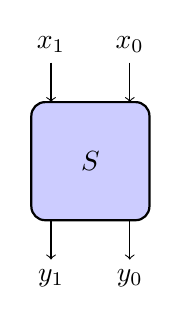
\begin{tikzpicture}

  % Box
  \draw[rounded corners=5pt, thick, fill=blue!20] (0,0) rectangle (1.5,1.5);
  
  % Text
  \node at (0.75,0.75) {$S$};
  
  % Input arrows and mathematical notations with subscripts
  \foreach \x/\notation in {0.25/ x_1, 1.25/ x_0} {
    \draw[->] (\x, 2) node[above]{$\notation$} -- (\x, 1.5);
  }
  
  % Output arrows and mathematical notations with subscripts
  \foreach \x/\notation in {0.25/ y_1, 1.25/ y_0} {
    \draw[->] (\x, 0) -- (\x, -0.5) node[below]{$\notation$};;
  }
  
\end{tikzpicture}
\end{figure}
\column{0.3\textwidth}
\pause
$
\displaystyle \left(\begin{array}{rrrrr}
1 & 1 & 1 & 1 & 1 \\
0 & 0 & 1 & 1 & x_{1} \\
0 & 1 & 0 & 1 & x_{0} \\
0 & 0 & 1 & 1 & y_{1} \\
1 & 0 & 1 & 0 & y_{0} \\
0 & 0 & 0 & 1 & x_{1} x_{0} \\
0 & 0 & 1 & 1 & x_{1} y_{1} \\
0 & 0 & 1 & 0 & x_{1} y_{0} \\
0 & 0 & 0 & 1 & x_{0} y_{1} \\
\rowcolor{tug!20}
0 & 0 & 0 & 0 & x_{0} y_{0} \\
0 & 0 & 1 & 0 & y_{1} y_{0}
\end{array}\right) 
$
\pause
\column{0.5\textwidth}
$
\displaystyle \left(\begin{array}{rrrrr}
1 & 0 & 0 & 0 & x_{1} x_{0} + x_{1} + x_{0} + 1 \\
0 & 1 & 0 & 0 & x_{1} x_{0} + x_{0} \\
0 & 0 & 1 & 0 & x_{1} x_{0} + x_{1} \\
0 & 0 & 0 & 1 & x_{1} x_{0} \\
\rowcolor{tug!20}
0 & 0 & 0 & 0 & x_{0} + y_{0} + 1 \\
\rowcolor{tug!20}
0 & 0 & 0 & 0 & x_{1} + y_{1} \\
\rowcolor{tug!20}
0 & 0 & 0 & 0 & x_{1} y_{1} + x_{1} \\
\rowcolor{tug!20}
0 & 0 & 0 & 0 & x_{1} x_{0} + x_{1} y_{0} + x_{1} \\
\rowcolor{tug!20}
0 & 0 & 0 & 0 & x_{1} x_{0} + x_{0} y_{1} \\
\rowcolor{tug!20}
0 & 0 & 0 & 0 & x_{0} y_{0} \\
\rowcolor{tug!20}
0 & 0 & 0 & 0 & x_{1} x_{0} + x_{1} + y_{1} y_{0}
\end{array}\right)  
$
\end{columns}
\pause
\begin{itemize}
  \item \verb|sage.crypto.sboxes.SBox.polynomials()|
\end{itemize}
\end{frame}

\section{Gr\"{o}bner Basis}
\sectionheader[\huge\color{tug}\faUniversity]{\marknotcovered
Gr\"{o}bner Basis}

\begin{frame}[fragile]
\frametitle{Ring of Multivariate Polynomials over a Finite Field}
\begin{itemize}
  \item $\mathbb{F}_{q}$ a finite field of order $q$
  \item Ring of multivariate polynomials over $\mathbb{F}_{q}$: $P = \mathbb{F}_{q}[x_{1}, \dots, x_{n}]$
  {\small\[
    P = \{\sum_{u} a_{u}x^{u} \,|\; n \in \mathbb N, a_{u} \in \mathbb{F}_{q}, \, u\in \mathbb{Z}_{\geq 0}^{n}\}
  \]}
  \vspace{-0.5cm}
  \item Monomial ordering: decides how we compare monomials
{\footnotesize
\begin{minted}[linenos]{python}
sage: P.<x, y, z> = PolynomialRing(GF(127), order='lex')
sage: f = P.random_element(); f
62*x*y - 29*y*z + 35*z^2 - 54*z - 55
sage: x*y > y^3 # variables then degree
True
sage: P.<x, y, z> = PolynomialRing(GF(127), order='deglex')
sage: x*y > y^3 # degree then variables
False
sage: f.monomials(), f.lm()
([x*y, y*z, z^2, z, 1], x*y)
\end{minted}
}
\end{itemize}
\end{frame}

\begin{frame}[fragile]
\frametitle{Ideals and Varieties}
\vspace{-0.3cm}
\begin{itemize}
  \small
  \item Ideal: $\mathcal{I} \subset P$, such that for all $f, g\in \mathcal{I}$, and all $h\in P$: $f + gh \in \mathcal{I}$
  \item $\langle f_{1}, \ldots, f_{m}\rangle$ is the ideal spanned by $F = \{f_{1}, \ldots, f_{m}\}$
  {\small\begin{equation*}
  \ideal(F) = \left\{\sum_{i=1}^{n} r_i \cdot f_i \midsized n \in \mathbb N, h_i \in R, f_i \in F\right\}.
  \end{equation*}}
  \item Variety of an ideal $\mathcal{I}$: $\mathcal{V}(\mathcal{I}) = \{x\in \mathbb{F}_{q}^{n} \mid f(x) = 0 \text{ for all } f\in \mathcal{I}\}$
  \item Zero-dimensional variety: Contains only finitely many points ($\dim(V) = 0$)
{\footnotesize
\begin{minted}[linenos]{python}
sage: P.<x, y, z> = PolynomialRing(GF(127), order='lex')
Defining x, y, z
sage: I = ideal(x*y + z, y^3 + 1, z^2 - 5*x - 1)
sage: (x*y + z) + P.random_element()*(y^3 + 1) in I
True
sage: I.variety()
[{z: 21, y: 108, x: 88}, {z: 6, y: 108, x: 7}]
\end{minted}
}
\end{itemize}
\end{frame}

\begin{frame}[fragile]
\frametitle{Ideal Membership in $\mathbb{F}_{q}[x]$}
\begin{itemize}
  \footnotesize
  \item Assume that $P = \mathbb{F}_{q}[x]$, and $I = \langle f \rangle$, where $f\in P$.
  Check if $f(x)\in I$.
  \item $\forall\, f(x), g(x) \in P\; \exists\, q(x), r(x) \in P\,:$ 
  \[g(x) = q(x)f(x) + r(x), \, \text{where}\, r = 0, \, \text{or} \, \deg(r(x)) < \deg(f(x))\]
  \vspace{-0.4cm}
  \item Divide $g(x)$ by $f(x)$. If $r(x) = 0$, then $f \in I$.
{\footnotesize
\begin{minted}[linenos]{python}
sage: P.<x> = PolynomialRing(GF(7))
sage: f, g = P.random_element(), P.random_element(degree=6); f, g
(4*x^2 + 4*x + 5
,3*x^6 + 6*x^5 + 4*x^4 + 4*x^3 + 2*x^2 + 6*x)
sage: I = Ideal([f])
sage: g // f, g%f, g in I
(2*x^3 + 5*x^2 + 2, 0, True)
\end{minted}
}
\item \textcolor{tugred}{What if we want to check if $g \in I = \langle f_{1}, \ldots, f_{m}\rangle$, where $g, f_{1}, \ldots, f_{m} \in P = \mathbb{F}_{q}[x_{1}, \ldots, x_{n}]$}?
\end{itemize}
\end{frame}

\begin{frame}[fragile]
\vspace{-0.5cm}
\frametitle{Ideal Membership in $\mathbb{F}_{q}[x_{1}, \ldots, x_{n}]$}
\begin{itemize}
  \item To check if $f \in \langle f_{1}, \ldots, f_{m} \rangle$ we follow the same idea.
  \item \textbf{Division Algorithm}: Represent $f$ in the form:
  \begin{itemize}
    \item \[f = q_{1}f_{1} + \cdots + q_{m}f_{m} + r, \, \text{where}\, r = 0\]
    \item $r = 0$, or no terms of $r$ is divisible by any of $\texttt{LT}(f_{1}), \ldots, \texttt{LT}(f_{m})$ 
  \end{itemize}
{\footnotesize
\begin{minted}[linenos]{python}
sage: P.<x, y> = PolynomialRing(GF(7), order='deglex')
sage: f1, f2 = x*y - 1, y^2 - 1
sage: f = x*y^2 - x
sage: f.reduce([f1]).reduce([f2])
-x + y
sage: f.reduce([f2]).reduce([f1])
0
\end{minted}
}
  \item \textcolor{tugred}{Remainder is not unique!} 
  \item We can not decide if $f \in \langle f_{1}, \ldots, f_{m} \rangle$ based on any basis.
\end{itemize}
\end{frame}

\begin{frame}[fragile]
\frametitle{Gr\"{o}bner Basis}
\begin{itemize}
  \item Let $I \subseteq P = \mathbb{F}_{q}[x_{1}, \ldots, x_{n}]$ be an ideal
  \item A Gröbner basis $G = \{g_{1}, \ldots, g_{t}\}$ for $I$ is a special basis:
  \begin{itemize}
    \item $f \,\%\, G$ is unique regardless of the order of elements in G
    \item It can solve the ideal membership problem: $f\in I\, \iff\, f\,\%\,G = 0$
  \end{itemize}
{\footnotesize
\begin{minted}[linenos]{python}
sage: P.<x, y> = PolynomialRing(GF(7), order='deglex')
sage: f1, f2 = x*y - 1, y^2 - 1
sage: I = ideal([f1, f2])
sage: f = x*y^2 - x
sage: g1, g2 = I.groebner_basis()
sage: f.reduce([g1]).reduce([g2]) == f.reduce([g2]).reduce([g1]) == 0
True
sage: f in I
True
\end{minted}
}
\end{itemize}
\end{frame}

\begin{frame}[fragile]
\frametitle{Gr\"{o}bner Basis and Solving System of Polynomial Equations}
\begin{itemize}
  \small
  \item $F = \{f_{1}, \ldots, f_{n}\}$ be a system of polynomial equations in $n$ variables
  \item $F$ is linear: Gaussian elimination
{\footnotesize
\begin{minted}[linenos]{python}
sage: P.<x, y, z> = PolynomialRing(GF(7), order='deglex')
sage: F = Sequence([-3*y + x, -2*x - y - 3*z + 2, x + y + 2*z - 1])
sage: A, v = F.coefficient_matrix()
sage: A.echelonize() # Echelon form
sage: (A*v).T
[x + 2, y + 3, z - 3]
\end{minted}
}
  \item Let us compute the Gr\"{o}bner basis of $F$:
{\footnotesize
\begin{minted}[linenos]{python}
sage: F.groebner_basis()
[x + 2, y + 3, z - 3]
\end{minted}
}
\item It is not by accident! Gr\"{o}bner basis generalizes row echelon form over $\mathbb{F}_{q}^{n}$
\end{itemize}
\end{frame}

\begin{frame}{Gröbner Basis - Generalizing Row Echelon Form I}
\vspace{-3mm}
\begin{block}{Reduced Gröbner Basis}
The reduced Gröbner basis \(G = \{g_1, g_2, \dots, g_{n}\}\) (in a specific term order) generating the zero-dimensional ideal \(I\) is of the form
\vspace{-3mm}
\[
G = 
\begin{cases}
g_1 &= x_1^{d} + h_1(x_1), \\
g_2 &= x_2 + h_2(x_1), \\
&\vdotswithin{=} \\
g_n &= x_n + h_n(x_1),
\end{cases}
\]
where \(h_i\) is a polynomial in \(x_1\) of degree at most \(d-1\).
\end{block}
\begin{itemize}
\item Note that \(g_1\) is now a univariate equation and we can solve it by factorization!
\item Use the result to solve for the other variables
\end{itemize}
\end{frame}

\begin{frame}[fragile]
\frametitle{Gr\"{o}bner Basis - Example}
\begin{itemize}
  \item Find the zeros (variety) of $I = \langle x + y + z, xy + xz + yz, xyz - 1 \rangle \subseteq \mathbb{F}_{127}[x, y, z]$
{\footnotesize
\begin{minted}[linenos]{python}
sage: P.<x, y, z> = PolynomialRing(GF(127), order='lex')
sage: I = ideal([x + y + z, x*y + x*z + y*z, x*y*z - 1])
sage: G = I.groebner_basis()
sage: for f in G: print(f)
x + y + z
y^2 + y*z + z^2
z^3 - 1
sage: V = I.variety(); V
[{z: 19, y: 1, x: 107},
  {z: 19, y: 107, x: 1},
  {z: 1, y: 19, x: 107},
  {z: 1, y: 107, x: 19},
  {z: 107, y: 19, x: 1},
  {z: 107, y: 1, x: 19}]
\end{minted}
}
\end{itemize}
\end{frame}

\begin{frame}[fragile]
\frametitle{Gröbner Basis - Systems with 0 or 1 Solution}
\begin{itemize}
  \item If the system has 1 solution:
  \[
  G = 
  \begin{cases}
  g_1 &= x_1 - a_1, \\
  g_2 &= x_2 - a_2, \\
  &\vdotswithin{=} \\
  g_n &= x_n - a_n,
  \end{cases}
  \]
  where $(a_{1}, \ldots, a_{n}) \in \mathbb{F}_{q}^{n}$
  \item If the system has no solution
  \[G = \langle 1 \rangle\]
\end{itemize}
\end{frame}

\begin{frame}{Gr\"{o}bner Basis - Complexity}
\begin{itemize}
  \item A fundamental tool in computational algebraic geometry (\textcolor{tugred}{1965}) \cite{PhD:Buchberger65}
  \item It solves the ideal membership problem and multivariate polynomial equations, and $\ldots$
  \item General algorithms, for any input system:
  \begin{itemize}
    \item Buchberger, F4, F5: They always terminate and give the Gr\"{o}bner basis
    \item But, the time is hard to predict for any instances
  \end{itemize}
  \item A hard problem:
  \begin{itemize}
    \item Ideal membership problem is an EXPSPACE-Complete problem
    \item Existence of solution to a system of polynomial equations over a finite field is NP-Complete \cite{fraenkel1979complexity}
  \end{itemize}
\end{itemize}
\end{frame}

\begin{frame}{Algebraic Cryptanalysis of \texttt{CTC} Block Cipher}
\vspace{-0.2cm}
\begin{itemize}
  \item \texttt{CTC} Block Cipher \cite{cryptoeprint_ctc1, cryptoeprint_ctc2}
\end{itemize}
\begin{figure}
\centering
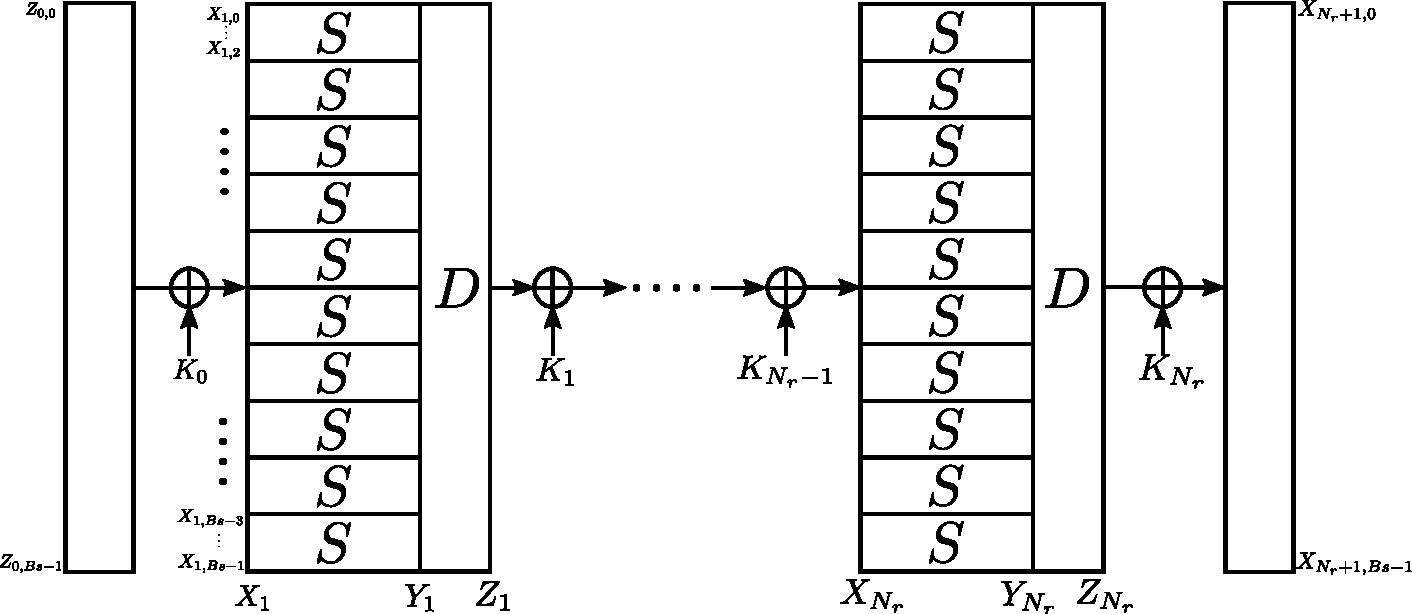
\includegraphics[width=0.9\textwidth]{./figures/AlgebraicAttacks/ctc.pdf}
\end{figure}
\begin{itemize}
  \item[\faGithub]\url{https://github.com/hadipourh/CTC2-Fast-Algebraic-Attack}
\end{itemize}
\end{frame}

%%% Summary %%%%%%%%%%%%%%%%%%%%%%%%%%%%%%%%%%%%%%%%%%%%%%%%%%%%%%%%

\begin{frame}{Algebraic Cryptanalysis -- Summary}
\begin{itemize}
\small
\item It is originally a deterministic Attack
\item Exploit the algebraic representation of cryptographic primitives
\item There are many approaches, we discussed only two:
\begin{itemize}
  \footnotesize
  \item Investigating the algebraic representation to find some weaknesses
  \item Expressing the cipher as a system of polynomial equations and solving it
\end{itemize}
\item We can take advantage of general-purpose solvers, e.g., Gr\"{o}bner basis, SAT, etc.
\item Work in many \emph{different fields} (\(\mathbb F_2\), \(\mathbb F_p\), \(\mathbb F_{2^n}\))
\end{itemize}
\end{frame}

%%% Questions %%%%%%%%%%%%%%%%%%%%%%%%%%%%%%%%%%%%%%%%%%%%%%%%%%%%%%

\begin{frame}{Questions}
\begin{enumerate}
\item What are some differences between statistical and algebraic attacks?
\item What is the core idea of the monomial prediction technique?
\item How does the monomial prediction technique help us find an integral distinguisher?
\item If certain variables corresponding to the secret key are absent in the ANF (Algebraic Normal Form) of the ciphertext bit, how can you exploit this to find a zero-sum distinguisher or use a cube attack?
\item Why can Gr\"{o}bner basis be used to solve systems of polynomial equations?
\end{enumerate}
\end{frame}

%%% BIBLIOGRAPHY %%%%%%%%%%%%%%%%%%%%%%%%%%%%%%%%%%%%%%%%%%%%%%%%%%%%
\unnumbered{
\begin{frame}[allowframebreaks]{Bibliography}
  \printbibliography
\end{frame}
}


%%% Backup Slides %%%%%%%%%%%%%%%%%%%%%%%%%%%%%%%%%%%%%%%%%%%%%%%%%%%
\begin{frame}[fragile]
  \frametitle{Convert \texttt{ANF} to \texttt{CNF}}
  \begin{itemize}
  \item By \texttt{ANF}-to-\texttt{CNF} conversion, we can use SAT solvers to solve (Boolean) polynomial equations:
  \begin{overprint}
  \scriptsize
  \begin{minted}[linenos]{python}
  sage: B = BooleanPolynomialRing(names=["a", "b", "c"]); B.inject_variables()
  Defining a, b, c
  sage: from sage.sat.converters.polybori import CNFEncoder
  sage: from sage.sat.solvers.dimacs import DIMACS
  sage: fn = tmp_filename(); solver = DIMACS(filename=fn)
  sage: e = CNFEncoder(solver, B)
  sage: e([a*b + a + 1, a*c + b])
  [None, a, b, c]
  sage: _ = solver.write()
  sage: print(open(fn).read())
  p cnf 3 5
  -2 0
  1 0
  -3 -1 2 0
  -2 1 0
  -2 3 0
  \end{minted}
  \end{overprint}
  \vspace{-0.2cm}
  \item A dedicated open-source tool: \href{https://github.com/meelgroup/bosphorus}{\texttt{Bosphorus}}
  \end{itemize}
  \end{frame}
  
\begin{filecontents*}[overwrite]{\jobname.bib}
@inproceedings{DBLP:conf/fse/JakobsenK97,
  author    = {Thomas Jakobsen and
               Lars R. Knudsen},
  title     = {The Interpolation Attack on Block Ciphers},
  booktitle = {{FSE}},
  series    = {Lecture Notes in Computer Science},
  volume    = {1267},
  pages     = {28--40},
  publisher = {Springer},
  year      = {1997}
}

@article{DBLP:journals/joc/NybergK95,
  author    = {Kaisa Nyberg and
               Lars R. Knudsen},
  title     = {Provable Security Against a Differential Attack},
  journal   = {J. Cryptology},
  volume    = {8},
  number    = {1},
  pages     = {27--37},
  year      = {1995}
}

@inproceedings{DBLP:conf/eurocrypt/CourtoisKPS00,
  author    = {Nicolas Courtois and
               Alexander Klimov and
               Jacques Patarin and
               Adi Shamir},
  title     = {Efficient Algorithms for Solving Overdefined Systems of Multivariate
               Polynomial Equations},
  booktitle = {{EUROCRYPT}},
  series    = {Lecture Notes in Computer Science},
  volume    = {1807},
  pages     = {392--407},
  publisher = {Springer},
  year      = {2000}
}

@phdthesis{PhD:Buchberger65,
  author       = {Bruno Buchberger},
  title        = {Ein Algorithmus zum Auffinden der Basiselemente des Restklassenringes nach einem nulldimensionalen Polynomideal},
  school       = {University of Innsbruck},
  year         = 1965,
}

@inproceedings{higherorderlai,
  title={Higher Order Derivatives and Differential Cryptanalysis},
  author={Xuejia Lai},
  booktitle={Communications and Cryptography 1994},
  pages={227--233},
  year={1994},
  publisher={Kluwer Academic Publishers}
}

@inproceedings{DBLP:conf/fse/Knudsen94,
  author    = {Lars R. Knudsen},
  title     = {Truncated and Higher Order Differentials},
  booktitle = {{FSE}},
  series    = {Lecture Notes in Computer Science},
  volume    = {1008},
  pages     = {196--211},
  publisher = {Springer},
  year      = {1994}
}

@misc{Keccak11,
 author = {G. Bertoni and J. Daemen and M. Peeters and G. Van Assche},
 title = {{The Keccak reference}},
 howpublished = {Round 3 submission to NIST SHA-3},
 year = {2011},
 url = {http://keccak.noekeon.org/Keccak-reference-3.0.pdf},
}

@article{DBLP:journals/iacr/Vielhaber07,
  author    = {Michael Vielhaber},
  title     = {Breaking {ONE.FIVIUM} by {AIDA} an Algebraic {IV} Differential Attack},
  journal   = {{IACR} Cryptology ePrint Archive},
  volume    = {2007},
  pages     = {413},
  year      = {2007}
}

@inproceedings{DBLP:conf/eurocrypt/DinurS09,
  author    = {Itai Dinur and
               Adi Shamir},
  title     = {{Cube Attacks on Tweakable Black Box Polynomials}},
  booktitle = {{EUROCRYPT} 2009},
  series    = {LNCS},
  volume    = {5479},
  pages     = {278--299},
  publisher = {},
  year      = {2009}
}

@inproceedings{DBLP:conf/eurocrypt/DinurMPSS15,
  author    = {Itai Dinur and
               Pawel Morawiecki and
               Josef Pieprzyk and
               Marian Srebrny and
               Michal Straus},
  title     = {Cube Attacks and Cube-Attack-Like Cryptanalysis on the Round-Reduced
               Keccak Sponge Function},
  booktitle = {{EUROCRYPT} {(1)}},
  series    = {Lecture Notes in Computer Science},
  volume    = {9056},
  pages     = {733--761},
  publisher = {Springer},
  year      = {2015}
}

@misc{cryptoeprint_ctc1,
      author = {Nicolas T.  Courtois},
      title = {How Fast can be Algebraic Attacks on Block Ciphers ?},
      howpublished = {Cryptology ePrint Archive, Paper 2006/168},
      year = {2006},
      url = {https://eprint.iacr.org/2006/168}
}

@misc{cryptoeprint_ctc2,
      author = {Nicolas T.  Courtois},
      title = {CTC2 and Fast Algebraic Attacks on Block Ciphers Revisited},
      howpublished = {Cryptology ePrint Archive, Paper 2007/152},
      year = {2007},
      url = {https://eprint.iacr.org/2007/152}
}

@article{fraenkel1979complexity,
  title={Complexity of problems in games, graphs and algebraic equations},
  author={Fraenkel, Aviezri S and Yesha, Yaacov},
  journal={Discrete Applied Mathematics},
  volume={1},
  number={1-2},
  pages={15--30},
  year={1979},
  publisher={Elsevier}
}

@inproceedings{monomial_prediction_asiacrypt_HuSW020,
  author    = {Kai Hu and
               Siwei Sun and
               Meiqin Wang and
               Qingju Wang},
  title     = {An Algebraic Formulation of the Division Property: Revisiting Degree
               Evaluations, Cube Attacks, and Key-Independent Sums},
  booktitle = {{ASIACRYPT} 2020},
  series    = {LNCS},
  volume    = {12491},
  pages     = {446--476},
  publisher = {Springer},
  year      = {2020},
  doi       = {10.1007/978-3-030-64837-4_15},
}

@inproceedings{sacrypt_BanikBIKLMSSS20,
  author    = {Subhadeep Banik and
               Zhenzhen Bao and
               Takanori Isobe and
               Hiroyasu Kubo and
               Fukang Liu and
               Kazuhiko Minematsu and
               Kosei Sakamoto and
               Nao Shibata and
               Maki Shigeri},
  title     = {{WARP}: Revisiting {GFN} for Lightweight 128-Bit Block Cipher},
  booktitle = {{SAC} 2020},
  series    = {LNCS},
  volume    = {12804},
  pages     = {535--564},
  publisher = {Springer},
  year      = {2020},
  doi       = {10.1007/978-3-030-81652-0_21}
}

@incollection{hod_discrete_derivatives_lai1994higher,
  author    = {Lai, Xuejia},
  title     = {Higher order derivatives and differential cryptanalysis},
  booktitle = {Communications and cryptography},
  pages     = {227--233},
  year      = {1994},
  publisher = {Springer}
}

@inproceedings{square_fse_DaemenKR97,
  author    = {Joan Daemen and
               Lars R. Knudsen and
               Vincent Rijmen},
  title     = {The Block Cipher {Square}},
  booktitle = {{FSE} 1997},
  series    = {LNCS},
  volume    = {1267},
  pages     = {149--165},
  publisher = {Springer},
  year      = {1997},
  doi       = {10.1007/BFb0052343},
}

@inproceedings{cansTodoA14,
  author    = {Yosuke Todo and
               Kazumaro Aoki},
  title     = {{FFT} Key Recovery for Integral Attack},
  booktitle = {{CANS} 2014},
  series    = {LNCS},
  volume    = {8813},
  pages     = {64--81},
  publisher = {Springer},
  year      = {2014},
  doi       = {10.1007/978-3-319-12280-9_5},
}

@inproceedings{sacryptSasaki012,
  author    = {Yu Sasaki and
               Lei Wang},
  title     = {Meet-in-the-Middle Technique for Integral Attacks against {Feistel}
               Ciphers},
  booktitle = {SAC 2012},
  series    = {LNCS},
  volume    = {7707},
  pages     = {234--251},
  publisher = {Springer},
  year      = {2012},
  doi       = {10.1007/978-3-642-35999-6_16},
}

@article{journals_istr_TehB22,
	author    = {Je Sen Teh and
		Alex Biryukov},
	title     = {Differential cryptanalysis of {WARP}},
	journal   = {J. Inf. Secur. Appl.},
	volume    = {70},
	pages     = {103316},
	year      = {2022},
	url       = {https://doi.org/10.1016/j.jisa.2022.103316},
	doi       = {10.1016/j.jisa.2022.103316}
}

@inproceedings{conf_space_KumarY21,
	author    = {Manoj Kumar and
		Tarun Yadav},
	title     = {{MILP} Based Differential Attack on Round Reduced {WARP}},
	booktitle = {{SPACE} 2021},
	series    = {LNCS},
	volume    = {13162},
	pages     = {42--59},
	publisher = {Springer},
	year      = {2021},
	doi       = {10.1007/978-3-030-95085-9_3},
}
\end{filecontents*}

\end{document}
